%!TEX root = ../terrainbook.tex

\graphicspath{{bathymetry/}}

\chapter{Processing bathymetric data to produce hydrographic charts}
\label{chap:bathymetry}

\begin{figure}[ht]
  \centering
  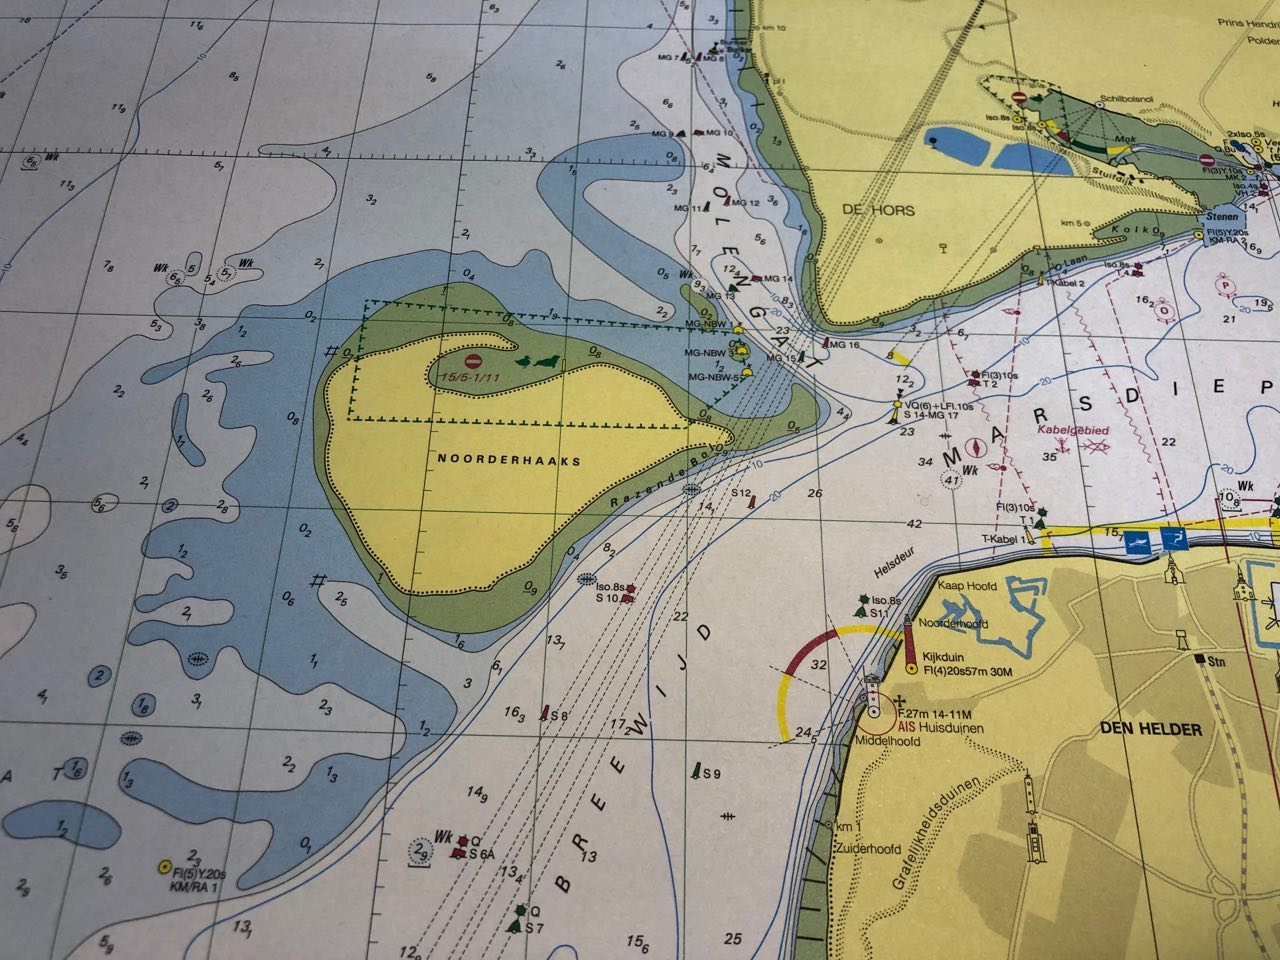
\includegraphics[width=0.8\linewidth]{figs/enc_denhelder.jpeg}
  \caption{An example of an ENC (electronic navigational chart) in the Netherlands. [photo of a paper map from the \emph{Hydrografische Dienst}]}
\label{fig:enc.jpg}
\end{figure}

An hydrographic chartis a map of the underwater world specifically intended for the safe navigation of ships.
In its digital form, it is often called an electronic navigational chart, or ENC.
The information appearing on an ENC are standardised.

%

We focus in this chapter on one element of these charts: depth-contours, which are akin to isocontours as seen in Chapter~\ref{chap:conversion} but show the depth with respect to a given level of water.

%

Traditionally, the depth-contours have been drawn by hand by skilled hydrographers.
They used a limited set of scattered surveyed depth measurements to deduct and depict the morphology of the seafloor with smooth-looking curves.



and still today it is often the case


%%%%%%%%%%%%%%%%%%%%
%
\section{Notes \& comments}



%%%%%%%%%%%%%%%%%%%%
%
\section{Exercises}

\begin{enumerate}
  \item Bacon ipsum dolour sit amet porchetta beef turkey, bacon turducken boudin hamburger venison ball tip. Brisket pork loin bresaola short loin ground round leberkas pastrami tongue jerky cow turducken beef ribs. Pork ribeye landjaeger prosciutto pig venison tenderloin. Swine beef ribs kielbasa, porchetta tenderloin salami venison pork belly tail.
  \item Bacon ipsum dolour sit amet porchetta beef turkey, bacon turducken boudin hamburger venison ball tip. Brisket pork loin bresaola short loin ground round leberkas pastrami tongue jerky cow turducken beef ribs. Pork ribeye landjaeger prosciutto pig venison tenderloin. Swine beef ribs kielbasa, porchetta tenderloin salami venison pork belly tail.
\end{enumerate}